\documentclass[conference]{IEEEtran}
\IEEEoverridecommandlockouts
% The preceding line is only needed to identify funding in the first footnote. If that is unneeded, please comment it out.
\usepackage[noadjust]{cite}
\usepackage{filecontents}
\usepackage{amsmath,amssymb,amsfonts}
\usepackage{algorithmic}
\usepackage{graphicx}
\usepackage{textcomp}
\usepackage{subcaption}
\def\BibTeX{{\rm B\kern-.05em{\sc i\kern-.025em b}\kern-.08em
    T\kern-.1667em\lower.7ex\hbox{E}\kern-.125emX}}
\begin{document}

\title{Landmarks detection by applying Deep networks}

%\author{\IEEEauthorblockN{Van Linh LE}
%\IEEEauthorblockA{\textit{LaBRI - CNRS 5800, France} \\
%\textit{ITDLU - Dalat University, Vietnam}\\
%van-linh.le@labri.fr/ \\
%linhlv@dlu.edu.vn}
%\and
%\IEEEauthorblockN{Marie BEURTON-AIMAR}
%\IEEEauthorblockA{\textit{LaBRI - CNRS 5800} \\
%\textit{Bordeaux University}\\
%Talence, France \\
%beurton@labri.fr}
%\and
%\IEEEauthorblockN{Akka ZEMMARI}
%\IEEEauthorblockA{\textit{LaBRI - CNRS 5800} \\
%\textit{Bordeaux University}\\
%Talence, France \\
%zemmari@labri.fr}
%\and
%\IEEEauthorblockN{Nicolas PARISEY}
%\IEEEauthorblockA{\textit{IGEPP} \\
%\textit{INRA 1349}\\
%Le Rheu, France \\
%nparisey@rennes.inra.fr}
%}

\maketitle

\begin{abstract}
Morphometric analysis is a general method applied to organisms and used to appreciate the covariances between the ecological factors and the organisms (shape, size, form,...) in which, landmark-based morphometry is known as one of the approaches to analyze the characteristics of organisms. Finding enough landmarks can give to biologists a comprehensive description of organism. In this study, we propose a convolutional neural network (CNN) to predict the landmarks on beetle images. The network is designed as a pipeline of layers, it was trained with a set of manually labelled landmarks dataset. Then, the network is used to provide the morphometric landmarks on biological images automatically. The coordinates of predicted landmarks are evaluated by computing the distance with the manual coordinates given by the biologists. Besides, The average of distance errors on each
landmark has been also given. The network is implemented by Python on Lasagne framework.
\end{abstract}

\begin{IEEEkeywords}
Morphometry, biological, landmarks, deep learning, convolutional neural networks
\end{IEEEkeywords}

\section{Introduction}
Morphometry analysis refers to measure the topography of an object, a notion that includes the shape and size. Morphometry analysis is often applied to biological organisms. Biologists work with several parameters from organisms such as lengths, widths, masses, angles,... to analyze the interaction of environment with organisms development. Besides the traditional information, landmarks (or points of interest in the image) are known as one of the characteristics to analyze the shape. Instead of collecting all information, the shape is determined by a finite set of points, called landmarks. The landmarks are the points that store the important information about the shape of the object, \textit{for example}, the corners of the human mouth are a kind of landmarks. Currently, the landmarks are along the outline of the object but in some special cases, it has been defined inside the object. Morphometry landmarks are a kind of points-of-interest, they are directly linked to the animal anatomy. In our study, the morphometric landmarks are specific points defined by the biologists. They are used in many biological studies. Manual landmarks setting is time-consuming and difficult to reproduce. Therefore, a method that gives automatically the location of landmarks could has a lot of interest.

This work introduces a method for automatic detection of the landmarks on biological images. The main idea consists design and train of  a convolutional neural network \cite{lecun2010convolutional} with a set of manual landmarks. By this way, the trained network will be able to detect the morphometry landmarks on biological images. The dataset includes 293 beetles images from Brittany lands. All the images are presented in RGB color with two dimensions. For each beetle, the biologists took images of five parts: \textit{left and right mandibles, head, body, and pronotum}. For each image, a set of landmarks has been manually determined by experts. In another work \cite{le2017maelab}, a method has been presented to determine the landmarks on left and right mandibles (Fig. \ref{figsub01}). This method is based on the image processing techniques \cite{canny1986computational}, combining with principal component analysis \cite{shlens2014tutorial} and SIFT descriptor \cite{lowe2004distinctive}. In the context of this work, we work on the dataset of pronotum images (Fig. \ref{figsub02}). For each pronotum image, a set of 8 manual landmarks have been set by the biologists. The coordinates of manual landmarks were used as the input to train the network. During the first phase, a number of 260 images and their manual landmarks were used to train and validate the network. The remaining images were used to evaluate the output model of the network in the second phase.

%\begin{figure}[htbp]
%	\centerline{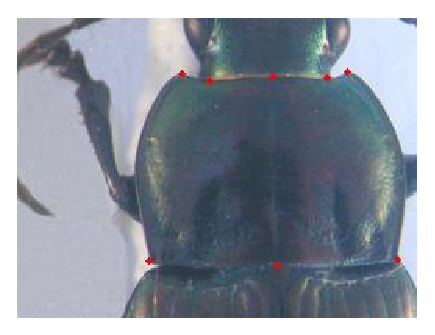
\includegraphics[scale=0.8]{images/pronotum}}
%	\caption{An example of pronotum with manual landmarks}
%	\label{figpronotum}
%\end{figure}
\begin{figure}[htbp]
    \centering
    \begin{subfigure}[t]{0.25\textwidth}
        \centering
        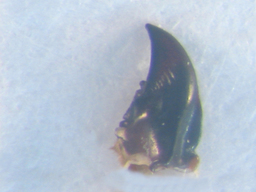
\includegraphics[height=1.2in]{images/md19}
        \caption{Right mandible}
        \label{figsub01}
    \end{subfigure}%
    ~ 
    \begin{subfigure}[t]{0.25\textwidth}
        \centering
        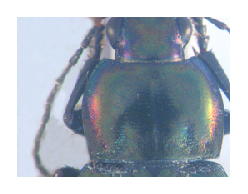
\includegraphics[height=1.2in]{images/prono60}
        \caption{Pronotum }
        \label{figsub02}
    \end{subfigure}
    \caption{An example of right mandible and pronotum image}
    \label{figsub012}
\end{figure}

In the next section, we present related works to determine the landmarks on 2D images by CNN. In section 3, we present an overview about convolutional neural networks. Section 4 presents the architecture of the network, its parameters, and the implementation. All the experiments and analysing the results are detailed in section 5.
\section{Related works}
Landmark or point of interest is a specific point that may contain the useful information. For example, the tip of the nose or the corners of the mouth are landmarks on human face. In image processing, we can consider two kinds of cases: the object of interest can or not be segmented. Setting landmarks can not be achieved in the same way depending on which situation we are. When segmentation can be applied, Lowe et al. \cite{lowe2004distinctive} have proposed SIFT method to find the corresponding keypoints between two images. Palaniswamy et al. \cite{palaniswamy2010automatic} have proposed a method based on probabilistic Hough Transform to automatically locate the landmarks in digital images of Drosophila wings. In our work \cite{le2017maelab}, we have proposed a method which have been extended from Palaniswamy's method, to determine landmarks on mandibles of beetles. The mandibles of beetle have the simple shape and easy to segment. We have obtained good enough results about determining the landmarks automatically on mandibles. Unfortunately, this method can not be applied to other parts of beetles than the pronotum seems is segmentation has too many noises.

In recent years, deep learning is known as a solution in computer vision. Using convolutional network to determine the landmarks on 2D images has achieved better results and it seems that good solutions for the images that can not segment. Yi Sun et al. \cite{sun2013deep} have proposed cascaded convolutional neural networks to predict the facial points of interest on the human face.
Zhanpeng Zhang et al. \cite{zhang2014facial} proposed a \textit{Tasks-Constrained Deep Convolutional Network} to optimize facial landmarks detection. The model determines the facial landmarks with a set of related tasks such as head pose estimation, gender classification, age estimation, face recognition, or facial attribute inference. In biology field, Cintas et al. \cite{cintas2016automatic} has introduced a network to predict the landmarks on human ears. After training, the network has the ability to predict 45 landmarks on human ears. In this way, we have applied CNN computing to work with pronotum landmarks.

%The cascade convolutional neural networks are separated into three levels. In the first level, the networks are designed to predict several landmarks together by covering the whole face; the networks in the second and the third level are used to predict each landmark on the face. They take the patches centered at the predicted positions of previous levels as input and try to improve the accuracy of predicted positions. Zhanpeng Zhang et al\cite{zhang2014facial} proposed a \textit{Tasks-Constrained Deep Convolutional Network} to optimize facial landmarks detection. The model determines the facial landmarks with a set of related tasks such as head pose estimation, gender classification, age estimation, face recognition, or facial attribute inference. Firstly, all the images are used as the input, their output spaces the images into several tasks. Then, the network is applied to determine the landmarks on the images of each task. In biology field, Cintas et al\cite{cintas2016automatic} has introduced a network to predict the landmarks on human ears. After training, the network has the ability to predict 45 landmarks on human ears. In their proposed architecture, the network with three times repeated of a structure includes two convolutional layers with the filters, followed by maximum pooling and dropout layers. The structures then adding two full-connected layers and a dropout layer. At the end, an output layer with 90 output units corresponding with 45 landmarks is hired to provide the position of the predicted landmarks.
\section{Convolutional neural networks}
Deep learning allows computational model composed of multiple processing layers to learn representations of data with multiple levels of abstraction \cite{lecun2015deep}. Each layer extracts the representation of the input data from the previous layer and computes a new representation for the next layer. In the hierarchy of model, higher layers of representation enlarge aspects of the input that is important for discrimination and suppress irrelevant variations. Each level of representations is corresponding to the different level of abstraction. During training, it uses gradient descent optimization method to update the learnable parameters via backpropagation. The development of deep learning opens promise results of the artificial intelligent on hight dimensional data, therefore applicable to many domains: image recognition and classification \cite{krizhevsky2012imagenet,ciregan2012multi,szegedy2015going}, speech recognition \cite{mikolov2011strategies,hinton2012deep,sainath2013deep}, question answering \cite{bordes2014question} and language translation \cite{sutskever2014sequence} \cite{jean2014using}.

Convolutional neural networks (CNNs) contribute to solve the state of the art in many computer vision tasks such as classification \cite{krizhevsky2012imagenet}\cite{ciregan2012multi} or recognition \cite{li2015convolutional}\cite{tompson2014joint}. A CNN consists a number of connected layers. The layers of CNN has neurons arranged in three dimensions: \textit{width, height, and depth} with learnable parameters. Fig. \ref{figconvarc} shows a common example of CNN. It is a pipeline of usual layers: convolutional layers (CONV), pooling layers (POOLING), dropout layers (DROPOUT), and full-connected layers (FC).
\begin{figure}[htbp]
	\centerline{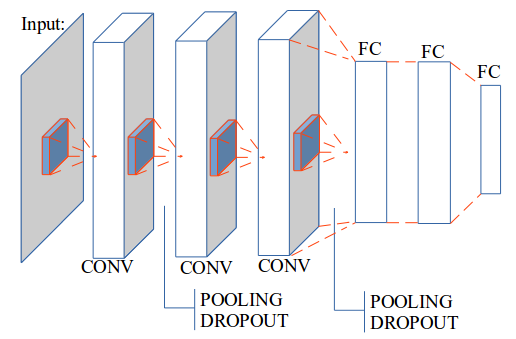
\includegraphics[scale=0.45]{images/convarc}}
	\caption{An example of usual convolutional neural network}
	\label{figconvarc}
\end{figure}

\textit{Convolutional} layer computes a dot product between their weights and a small region in the input. At the output, the results of connected local regions are combined. Convolution layer uses a set of learnable filters as parameters. Each filter is small spatially but extends the depth of the input. \textit{Pooling} layer is used to down-sampling the input, reduce the computational cost in remaining layers, and control overfit. \textit{Dropout} layer refers to dropping out units in the network. By dropping a unit out, we mean temporarily removing it from the network, along with all its incoming and outgoing connections. \textit{Full connected} layer refers to the output of the network. The number of outputs of the last full-connected layer are corresponding with the number of predicted values.

From the beginning of deep learning until now, many deep learning frameworks have been developed. Almost the framework was open source. According to the written programming languages, the frameworks can be separated into two main groups: C++, \textit{such as Caffe, Deeplearning4j, Microsoft Cognitive Toolkit} and Python \textit{i.e Keras, Theano, PyTorch}.  However, along with the development of deep learning, the frameworks support to design the network with other languages.
%In the group written by C++, the outstanding frameworks include Caffe\cite{jia2014caffe}, Deeplearning4j, Microsoft Cognitive Toolkit\cite{yu2014introduction}; whereas Keras\cite{chollet2015keras}, Theano\cite{2016arXiv160502688short} and more recently PyTorch\cite{} are known as the "noi bat" frameworks that implemented by Python.

Theano is an open source framework developed by machine learning group at the University of $Montr\acute{e}al$. It is a Python library that allows to define, optimize and evaluate mathematical expressions relating multi-dimensional arrays efficiently by using a Numpy package. Theano supports compiled on either CPU or GPU architectures. Lasagne \cite{lasagne} is a lightweight library in Theano. It allows to build and train the neural networks. In this work, we have used Lasagne to implement the proposed neural network. Recently, Theano has been stopped to develop but its community is still large. The networks which have been designed by Theano are still good to use in deep learning.
\section{Application to landmarks identification}
In previous sections, we have had an overview of the landmarks and CNN. In this section, we describe the designing processes of the model. We have also presented the data preprocessing, training and evaluating the model.
\subsection{Preprocessing data}
The images come from a collection of 293 beetles from Brittany lands. All the images are taken with the same camera under same conditions with a $3264 \times 2448$ resolutions. For each specific part, a set of manual landmarks has been determined by biologists, \textit{for examples, 8 landmarks for pronotum, 16 landmarks for the left mandible, 18 landmarks for right mandible}. In the content of this study, we work on pronotum part of beetle. The provided dataset contains 293 images, each image with 8 landmarks provided by biologists. The dataset was split into a training set with 260 images (training and validation) and a testing set of 33 images. During the training, the network learned the information through a pair of \textit{(image, landmarks)} in training set. At the testing phase, the image without landmarks was given to the trained network and the predicted landmarks will be given at the output. Fig. \ref{figpronotum} shows an example of pronotum image with its manual landmarks.

\begin{figure}[htbp]
	\centerline{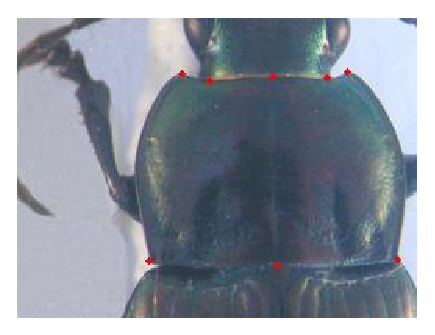
\includegraphics[scale=0.8]{images/pronotum}}
	\caption{An example of pronotum with manual landmarks}
	\label{figpronotum}
\end{figure}

In some succeed networks \cite{krizhevsky2012imagenet}\cite{sun2013deep}\cite{cintas2016automatic}, the maximum size of the inputs is not over 256 pixels. In our case, the resolution of the image is large, it becomes a difficulty for the network. During training and testing, the images are down-sampling to the new resolution of $256 \times 192$. Certainly, the landmark coordinates of the image are also scaled to suit their new resolution. 

The proposed network has a large number of learnable parameters. In addition, the size of the dataset is limited, this means that overfitting will occur during the training process. Therefore, we need to enlarge the size of the dataset. In image processing, we usually apply transform procedure (i.e rotate, translate) to generate a new image but in fact, when we compute the value of the pixels, it does not change while CNN computes the values of the pixels.Therefore, we have applied two other procedures to increase the number of images in the dataset. To address this problem, we have applied two procedures to enlarge the size of the dataset.

The first procedure was applied to change the value of each channel in the original image. According to this, a constant is added to a channel of RGB image and for each time, we just change the value of one of three channels. For example, from an original RGB image, if we add a constant $c = 10$ to the red channel, we will obtain a new image with the values at red channel by greater than the red channel of original image a value of 10. By this way, we can generate three new RGB images from a RGB image.

The second procedure is splitting the channels of RGB images. It means that we separate the channels of RGB into three gray-scale images. This work seems promising because the network works on single-channel images. At the end, we can generate six versions from an image, the total number of images used to train and validate is $260 \times 7 = 1820$ images (six versions and original image). The number of images that used for training and validation is splitted randomly by a ratio (training: $80\%$, validation: $20\%$) that has been set during the network setup.

In practical, when we work with CNN, convergence is usually faster if the average of each input variable over the training set is close to zero. Moreover, when the input is set closed with zero, it will be more suitable with the sigmoid activation function \cite{lecun2012efficient}. According to \cite{lecun2012efficient}, the brightness of the image is normalized to $[0,1]$, instead of $[0,255]$ and the coordinates of the landmarks are normalized to $[-1,1]$, instead of $[0,256]$ and $[0,192]$ before giving to the network.
\subsection{Network architecture and training}
Three networks have been proposed and trained to perform the best architecture for automatically landmarking predictions. The networks consist on several common layers in the neural network with different learnable parameters They receive the same input of $1 \times 256 \times 192$ to train but they have different number of layers. In this section, we introduce the architectures of the networks and the process to improve the architecture from the beginning of designing.

Fig. \ref{figarch0} shows the architecture of the first network. This model has been designed from a generic method: the layers in the network are very common as the other neural networks. The network consists on three repeated-structure of a convolutional layer followed by a maximum pooling layer. The depth of convolutional layers increases from $32, 64,$ and $128$ with different size of the filter kernel: $3 \times 3$, $2 \times 2$, and $2 \times 2$. All the kernels of pooling layers have the same size of $2 \times 2$.  At the end, three full connected layers have been added to the network. The outputs of the full connected layers are $500, 500,$ and $16$, respectively. The output of the last full-connected layer corresponds to 8 landmarks ($x$ and $y$ coordinates) which we would like to predict. The training result shows that the architecture of this model is not good enough to solve the problem. It is still simple and overfitting has appeared during training and validation. 

The second network has the same architecture as the first one. But, number of outputs at full-connected layers have been modified from $500$ to $1000$ (the second model) to prevent the overfitting, but the result did not lead to better performances. 
%The CNN was designed and trained for performing an automatic landmarks detection on pronotum images. The network consists several common layers in the neural network with different learnable parameters. It takes a single channel pronotum image with the size of  $256 \times 192$ as the input. Before entering the network, the brightness of pixels in the image are normalized to $[0,1]$ and the coordinates of landmarks are normalized to $[-1,1]$.

\begin{figure}[htbp]
	\centerline{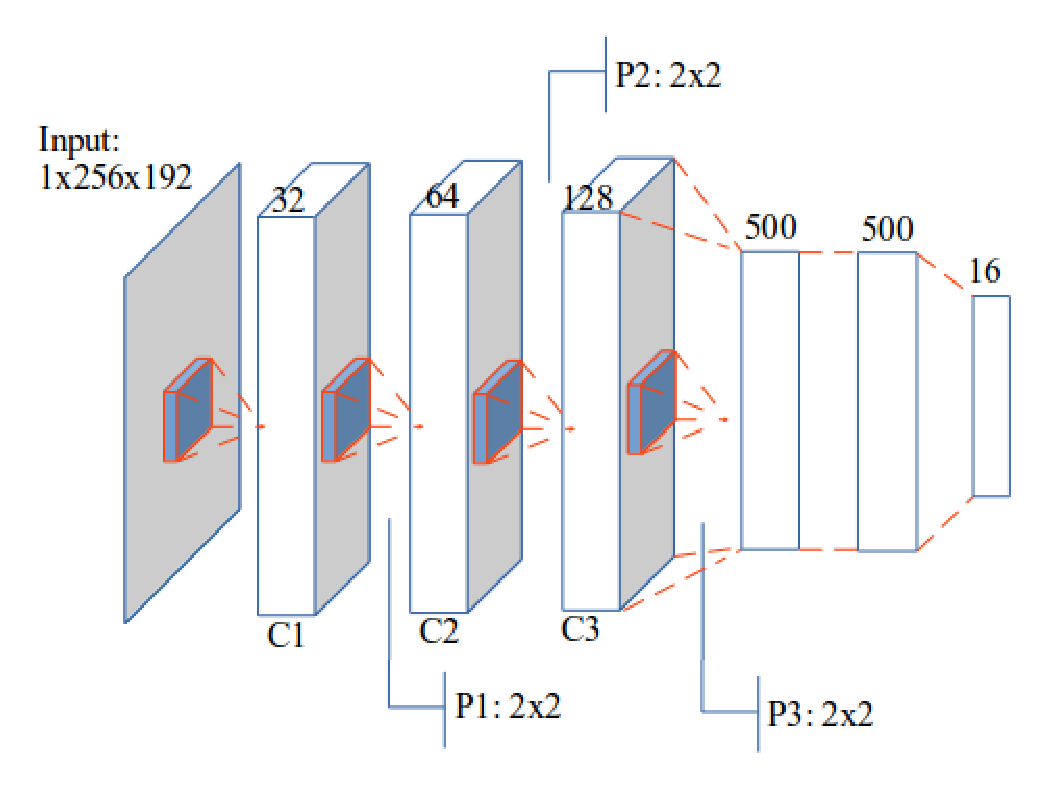
\includegraphics[scale=0.45]{images/architecture1}}
	\caption{The architecture of the first network}
	\label{figarch0}
\end{figure}

In the third network, instead of changing the parameters, we have added four dropout layers to the network. These are considered as the good solution to prevent the overfitting. The idea of dropout is to randomly drop units from the neural network during training. It prevents units from co-adapting too much. During training, dropout samples are done from an exponential number of different ``thinned" network. At test times, it is easy to approximate the effect of averaging the prediction of all thinned networks by simply using a single unthinned network with smaller weights. This significantly reduces overfitting and gives major improvements over other regularization methods \cite{srivastava2014dropout}. Fig.\ref{figarch} shows the architecture of the third network. The first three dropout layers are supplemented to the repeated-structures followed the maximum pooling layers. In that way, structure becomes a convolution layer with square filter, followed by a \textit{maximum} pooling and dropout layer. The probability values used for dropout layers are $0.1$, $0.2$, and $0.3$. Actually, we keep the same value for the parameters of the convolutional ($32, 64,$ and $128$), pooling ($3 \times 3$, $2 \times 2$, and $2 \times 2$) and full-connected layers ($1000, 1000,$ and $16$) as the second one.

\begin{figure}[htbp]
	\centerline{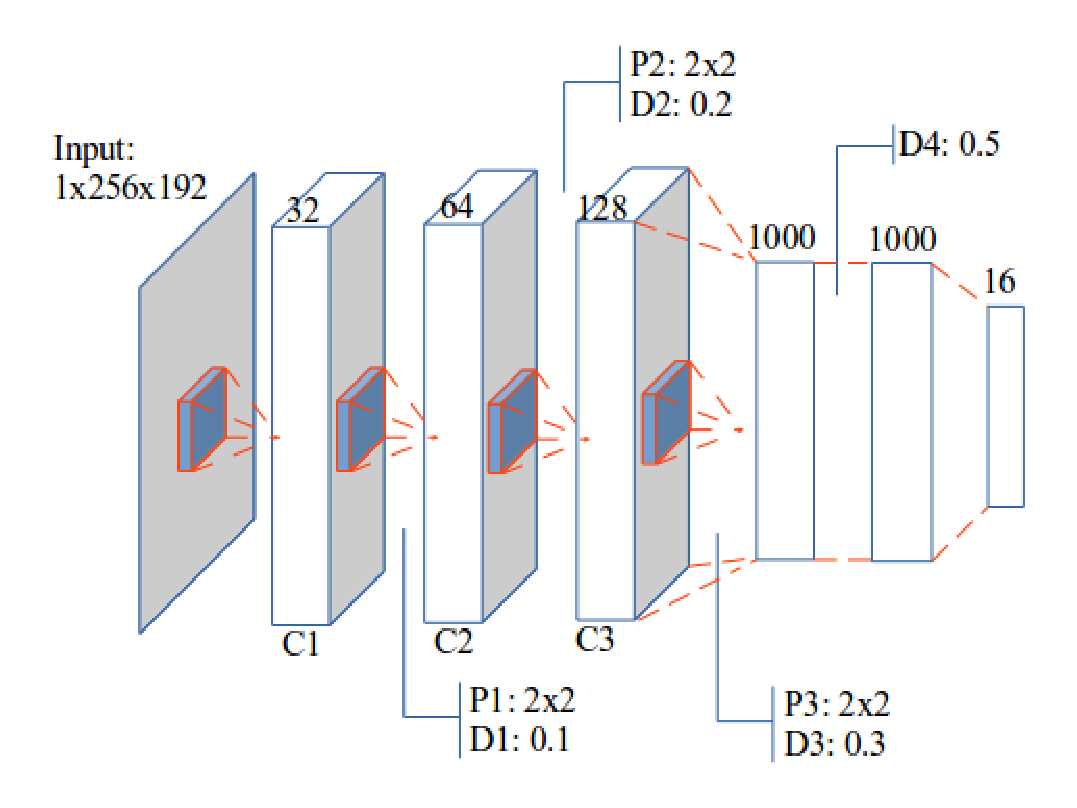
\includegraphics[scale=0.45]{images/architecture3}}
	\caption{The architecture of the last network}
	\label{figarch}
\end{figure}

The remaining dropout layer is inserted between the first two full connected layers. The probability value of this layer is set to $0.5$. The output layer still contains $16$ units corresponding to the coordinates of $8$ predicted landmarks.% The detail of parameters at each layer are shown in Appendix section. 

Additionally, the network is designed with a small sharing learning rate and the momentum. As usual, they have been used to perform gradient descent during backward phase to update the parameters of the layers. The value of learning rate and momentum are updated over training time to fit with the remaining number of iterations. The implementation of this architecture used Python on Lasagne framework \cite{lasagne} which allows to train the network on GPU. The training process took around 3 hours using NVIDIA TITAN X cards. The design of the network is available on GitHub\footnote{It is freely obtained by request the authors.}.
\subsection{Results}
The dataset has been built by the biologists. It includes the images and manual landmarks. So, we can use the manual landmarks coordinates as ground truth to evaluate the coordinates of predicted landmarks. In the context of deep learning, landmark prediction can be seen as a regression problem. Therefore, the quality metric is used to evaluate the results. In particular, we use root mean square error (RMSE) to compute the accuracy of the implemented architecture. 
\begin{figure}[h!]
	\centerline{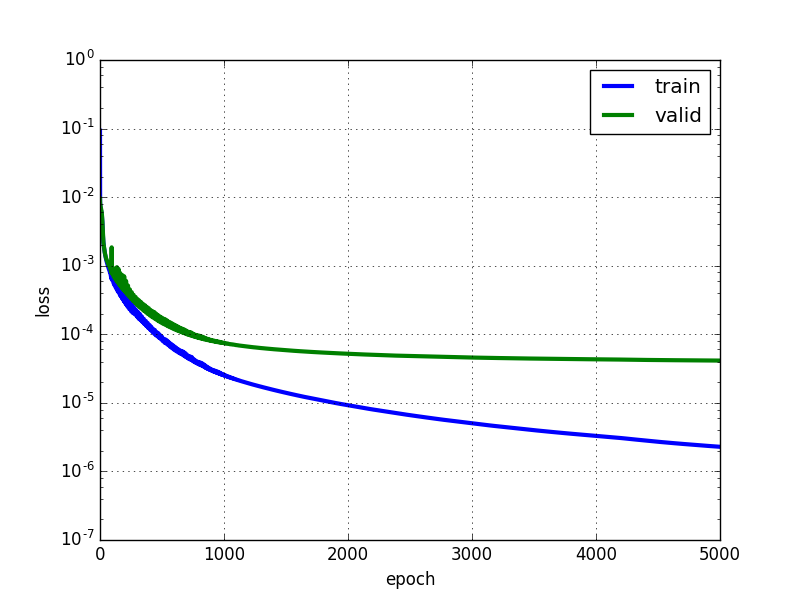
\includegraphics[scale=0.45]{images/loss_model_1}}
	\caption{Learning curves of the first model.}
	\label{figloss1}
\end{figure}~\\
\begin{figure}[h!]
	\centerline{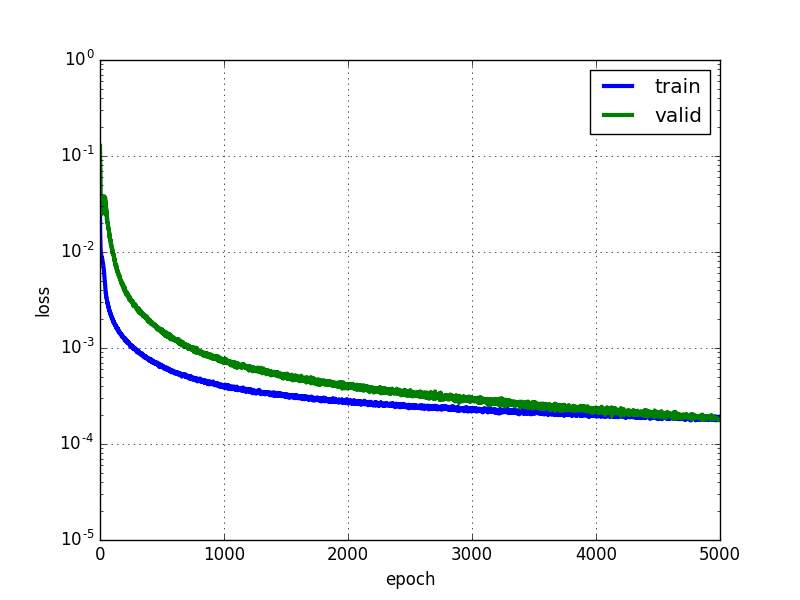
\includegraphics[scale=0.45]{images/loss_v16}}
	\caption{Learning curves of the last model.}
	\label{figloss}
\end{figure}~\\[0.1cm]
Fig.\ref{figloss1} and \ref{figloss} show the training errors and the validation errors of a training time on the first and the third model, respectively. The blue curve presents RMSE on training set, the green curve presents the validation error. Clearly, the overfitting has appeared in the first model. In Fig.\ref{figloss1}, we can see that if the training is able to decrease with the number of epochs\footnote{An epoch is a single pass through the full training set.}, it is not the case of validation loss. At the opposite in the third model, we can see some different values for the two losses at the beginning but after several epochs, these values become more proximate and the overfitting problem has been solved.

Fig.\ref{figrsexample} shows the predicted landmarks on test images set by the thrid model. When we consider the distance between the predicted and manual landmarks, the accuracy on coordinates of predicted landmarks on Fig.\ref{figsub1} is $99\%$. The propotion on Fig.\ref{figsub2} is $80\%$.

\begin{figure}[h]
    \centering
    \begin{subfigure}[t]{0.25\textwidth}
        \centering
        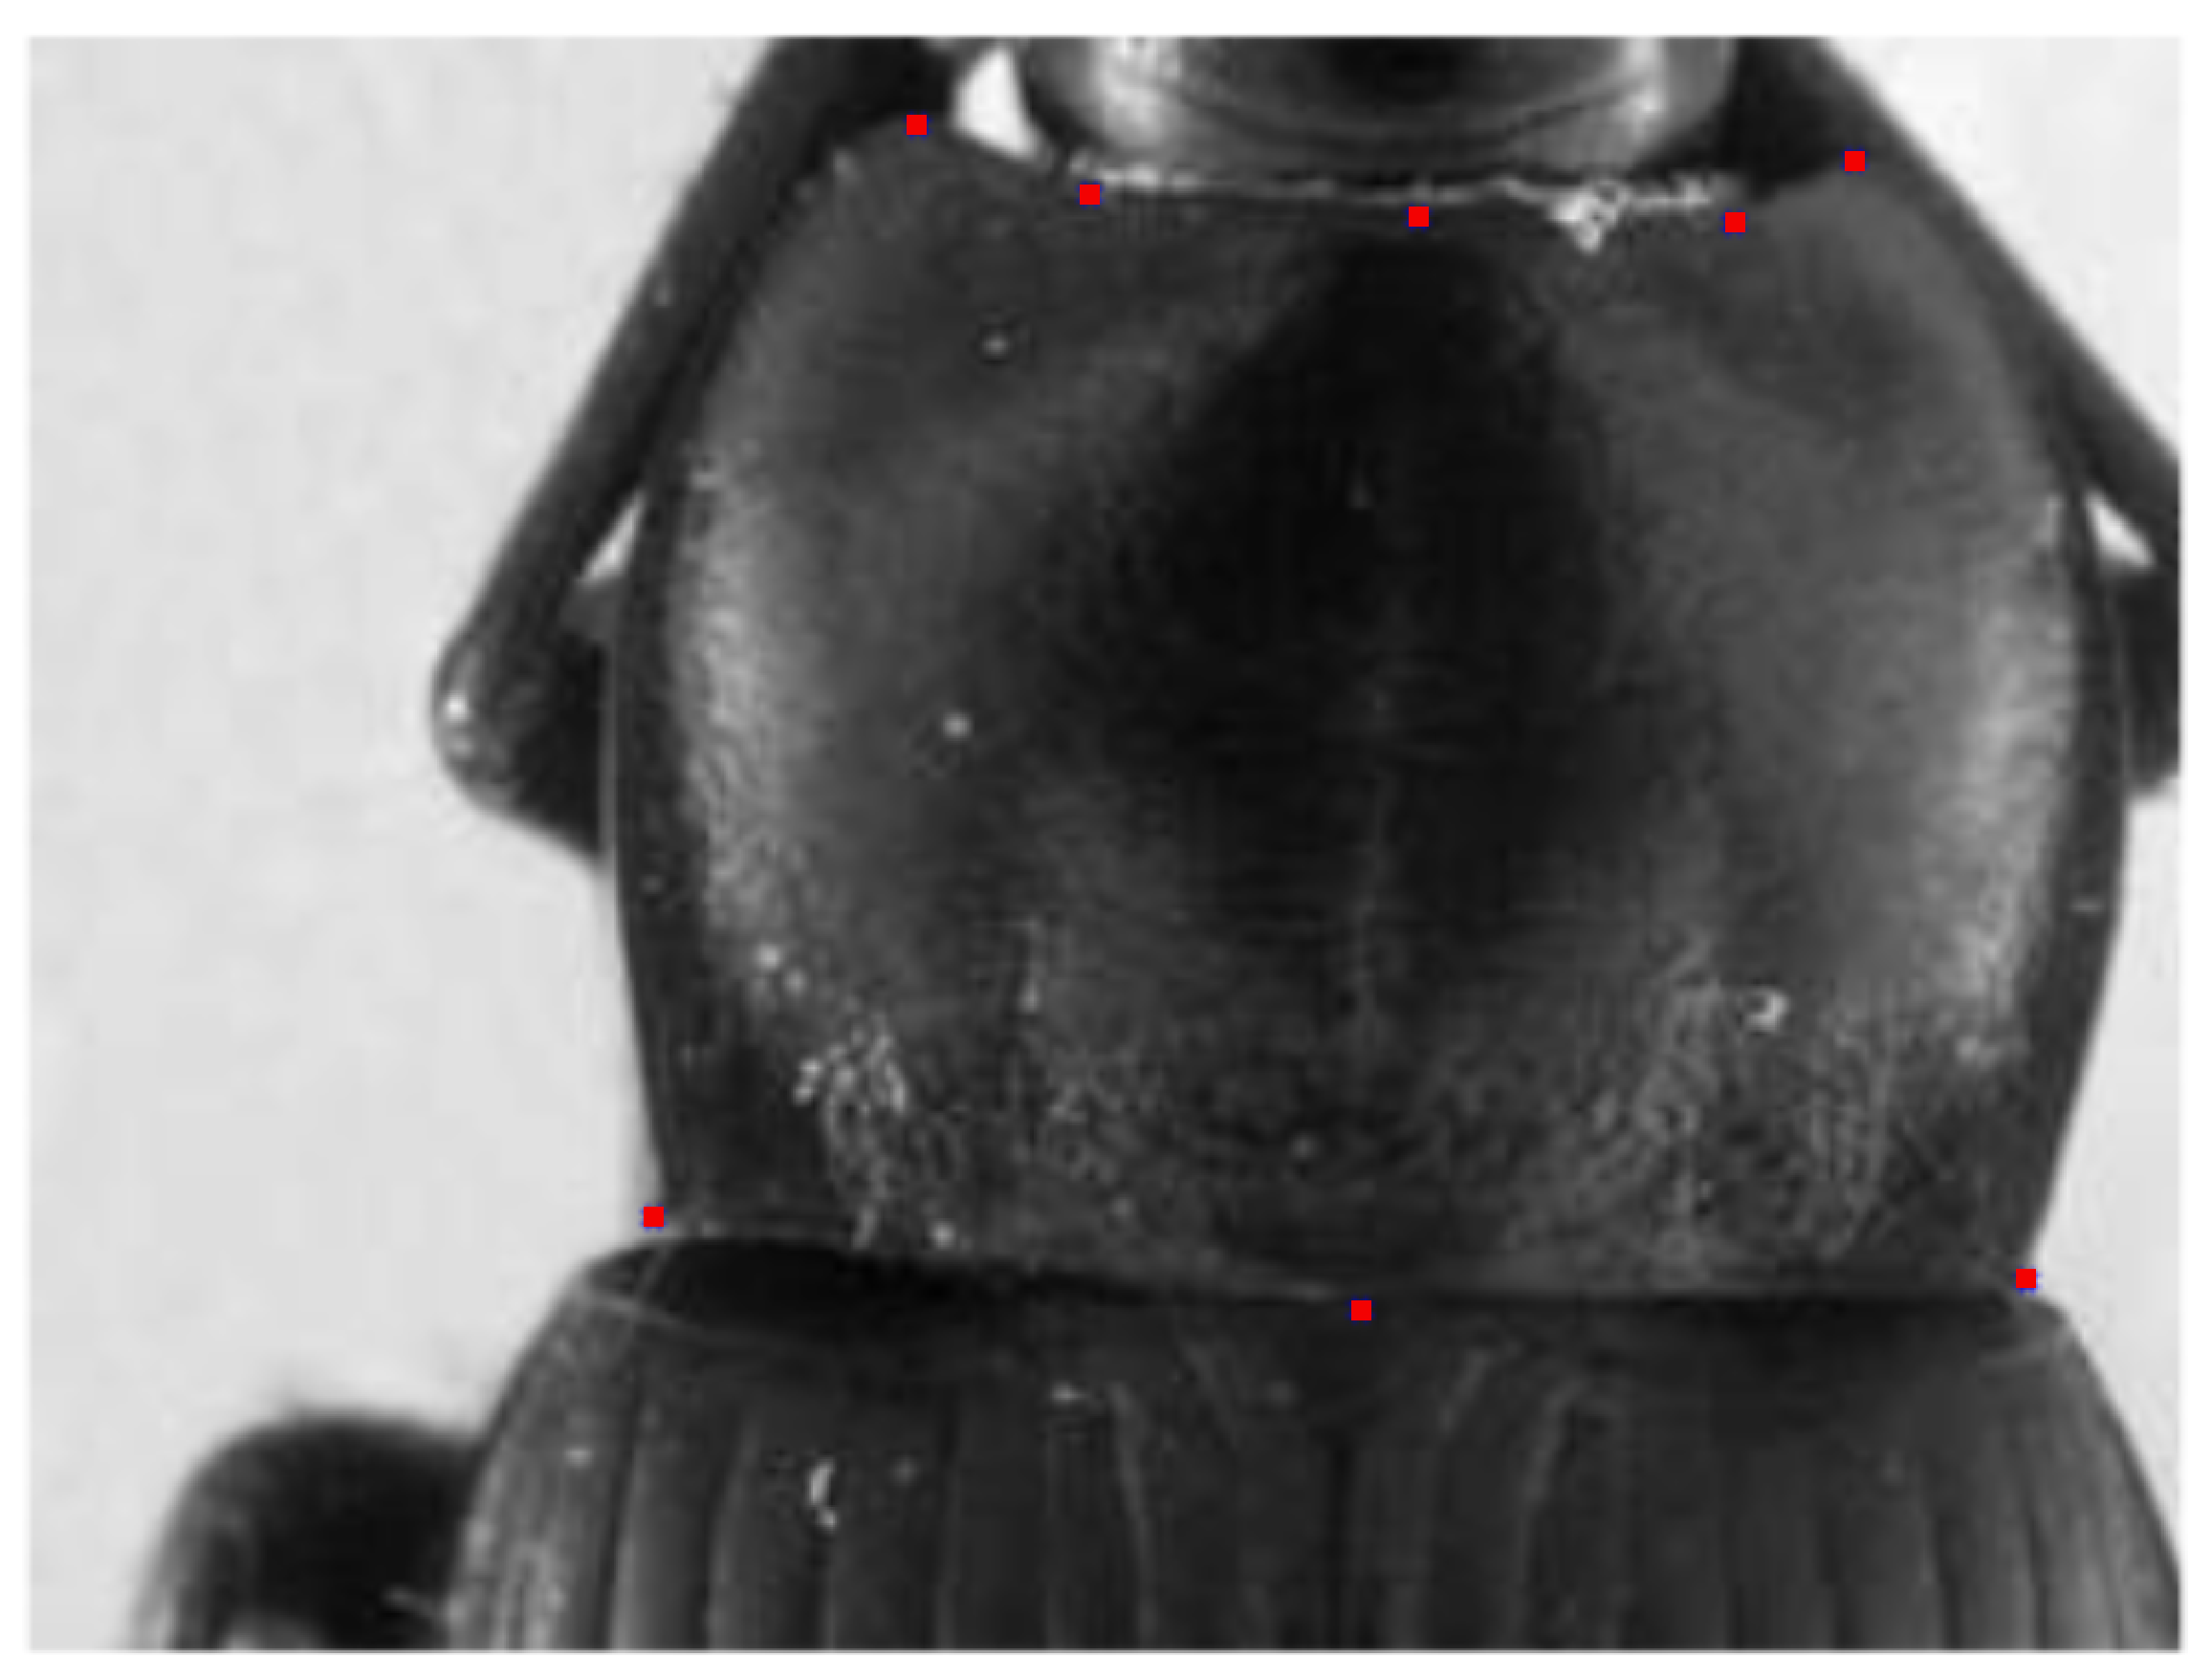
\includegraphics[height=1.2in]{images/plandmark}
        \caption{Image with well-predicted landmarks}
        \label{figsub1}
    \end{subfigure}%
    ~ 
    \begin{subfigure}[t]{0.25\textwidth}
        \centering
        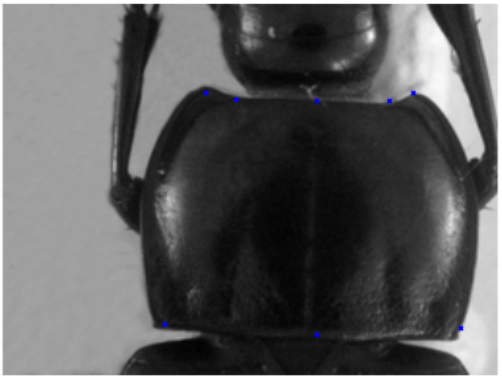
\includegraphics[height=1.2in]{images/plandmark2}
        \caption{Image with inaccuracy landmarks}
        \label{figsub2}
    \end{subfigure}
    \caption{The predicted landmarks on an image in test set (red points)}\
    \label{figrsexample}
\end{figure}
Besides the losses of training, the distance from predicted landmarks to manual landmarks of the test images deserve attention also. Firstly, the distance between them is calculated. Then, the standard deviation \cite{bland1996statistics} is used to quantify the dispersion of a set of distances. Table.\ref{tab2} shows the average error distance given on each landmark.

\begin{table}[htbp]
\caption{The average distance per landmark}
\begin{center}
\begin{tabular}{|c|p{1.5cm}|}
\hline
\textbf{$\#$Landmark} & \textbf{Distance} \\ \hline
1 & 4.002  \\ \hline
2 & 4.4831 \\ \hline
3 & 4.2959 \\ \hline
4 & 4.3865 \\ \hline
5 & 4.2925 \\ \hline
6 & 5.3631 \\ \hline
7 & 4.636 \\ \hline
8 & 4.9363 \\ \hline
\end{tabular}
\label{tab2}
\end{center}
\end{table}

Fig.\ref{figchartlm1} shows the distribution of the distances on the first landmarks of all images. The accuracy based on the distance of each image can be separated into three spaces: the images have the distance less than average value ($4$ pixels): \textbf{56.66$\%$}; the images have the distance from average value to $10$ pixels: \textbf{40.27$\%$}; and the images have the distance greater than $10$ pixels: \textbf{3.07$\%$}. The network has enabled to detect the landmark on pronotum automatically. %If we consider the distance less than average value are good,

\begin{figure}[htbp]
	\centerline{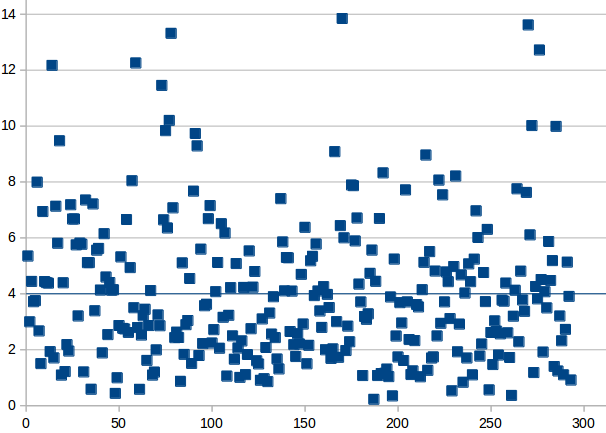
\includegraphics[scale=0.3]{images/statistic}}
	\caption{The distribution of the distances on the first landmark. The blue line is the average value of all distances.}
	\label{figchartlm1}
\end{figure}
Fig.\ref{figchart} shows the proportion of acceptable landmarks. In our case, a predicted landmark is acceptable if the distance between it and corresponding manual landmarks is less than the average distance plus a value of standard deviation. Most of the landmarks have been detected with the accuracy greater than $70\%$. %However, we can see a vast difference between the correlation coefficient results and the proportions on each landmark.

\begin{figure}[htbp]
	\centerline{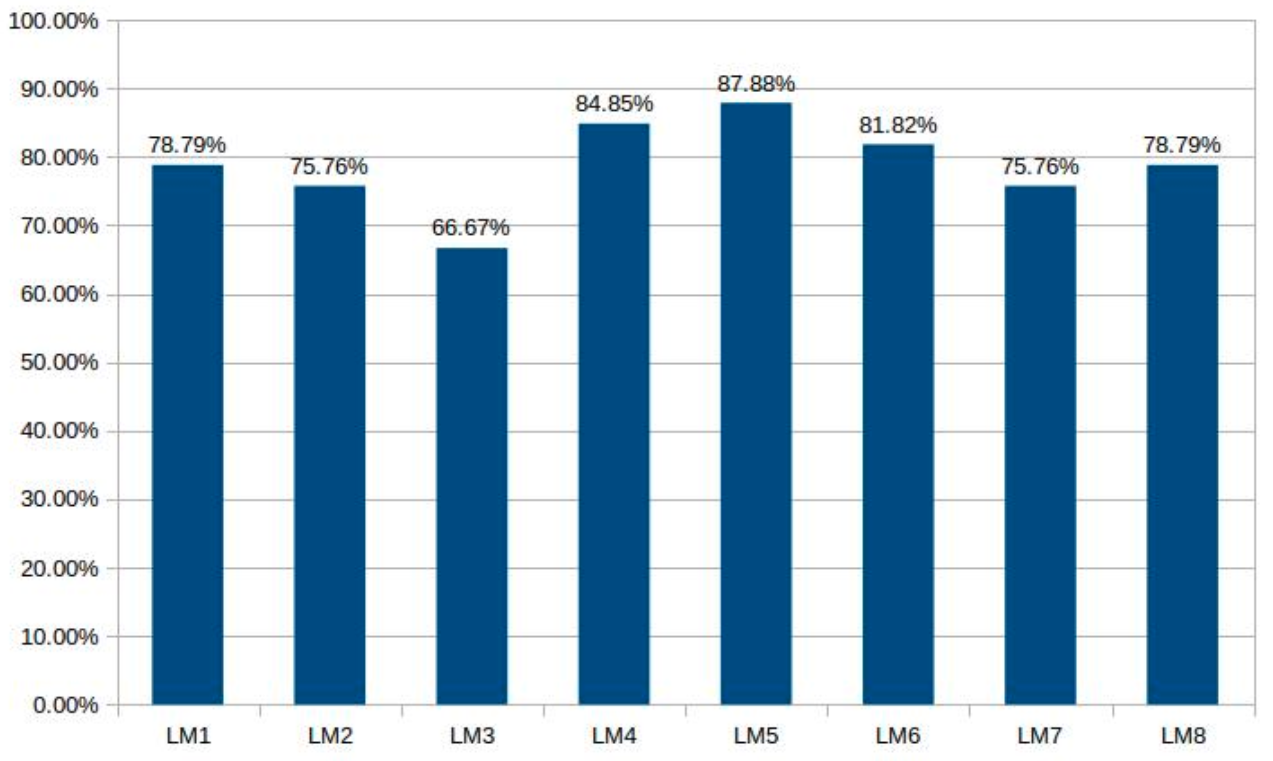
\includegraphics[scale=0.2]{images/chart}}
	\caption{The proportion of acceptable predicted landmarks}
	\label{figchart}
\end{figure}

At the test phase, the trained network is used to predict the landmarks on a set of test images. The program outputs the predicted-landmarks of the images as TPS files; in additional, it also fills and displays the predicted-landmarks on sixteenth firstly images of test data. With the outputs are TPS files, the user can use MAELab \cite{le2017maelab} framework\footnote{MAELab is a free software written in C++. It can be directly
and freely obtained by request at the authors.} to display the landmarks on the images.
\section{Conclusion and future works}
With beetle mandibles images, the object is easy to segment and we have succeeded to determine the landmarks automatically. In opposite, the pronotum images are difficult to segment. Methods which not suppose to be based on segmentation are necessary. In this paper, after testing several models, we have presented a convolutional neural network for automatic detection landmarks on the pronotum. It includes three times repeated structure which consists of a convolutional layer, a max pooling layer, and a dropout layer, followed by the connected layers. During the training phase, suitable techniques are used to prevent overfitting, a common issue of the neural networks. The network was trained several times in different selections of training data. After training with the manual landmarks given by the biologist, the network is able to predict the landmarks on the set of unseen images.

The results from the test set have been evaluated by calculating the distance between manual landmarks and corresponding predicted-landmarks. The average of distance errors on each landmark has been also considered. Using the convolutional network to predict the landmarks on biological images is promising good results in the case that the image can not be segmentation. The quality of prediction allows using automatic landmarking to replace manual landmarks in some aspects.  In our case, the training dataset is limited. As a result, the accuracy of the network is acceptable. However, when we expect more about the accuracy of predicted landmarks (coordinates of predicted landmarks), the result of this work is still needed to improve (for example using a larger training dataset). Therefore, future research in landmarking identification appears as an improved of the worth exploring.
%\section*{Acknowledgment}
%The research has been supported by INRA. We would like to thank the biologists, who have provided the dataset. We thank also our colleague, Nicolas PARISEY, who provided insight and expertise that greatly assisted the research.
\bibliographystyle{IEEEtran}
\bibliography{includes/references}
\end{document}
